\section{EpToTester}
\label{sec:epto}
\begin{figure}[htp]
	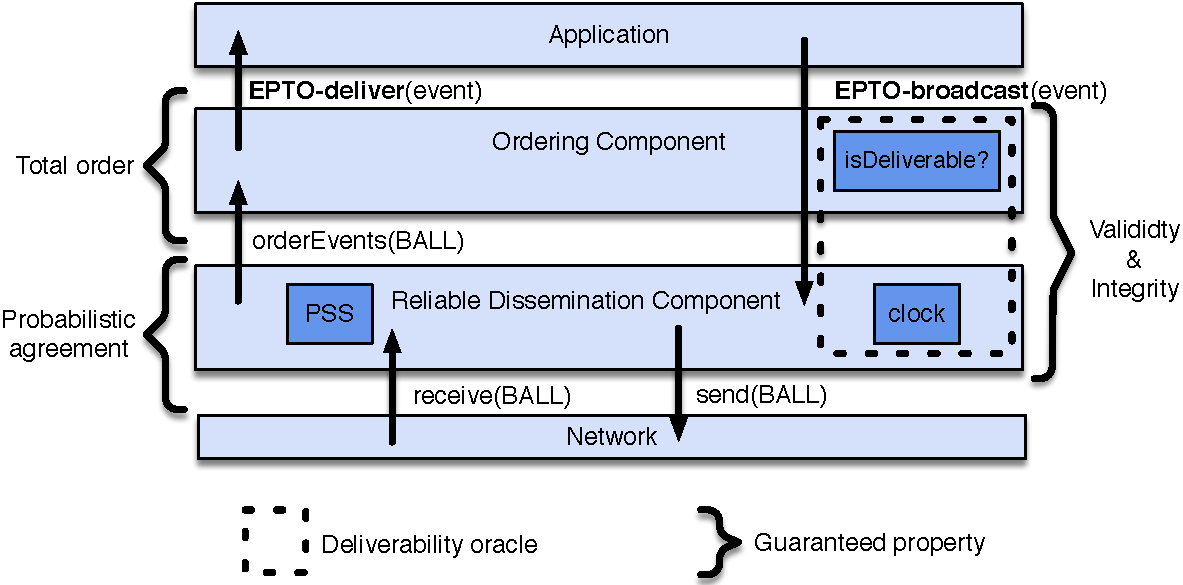
\includegraphics[width=\linewidth]{figures/architecture.pdf}
	\caption{\epto architecture \autocite{matos2015epto}.}
	\label{fig:epto-architecture}
\end{figure}
EpTOTester is a practical implementation of \epto designed to assess the claims made in \autocite{matos2015epto}. Although the implementation was written with benchmarking in mind, the code could be adapted to be used in a real application with only minimal changes to the sources.
\subsection{Architecture}
\autoref{fig:epto-architecture} illustrates the architecture of a single replica. An application extending our Application class can \epto-broadcast and \epto-deliver events. Events broadcasted to the Dissemination component are sent over the network every $\delta$ period. Every ball received from the network is unwrapped and its events are analyzed by the Dissemination component to find out whether they need to be propagated further or not according to their Time To Live (TTL). They are then sent to the ordering component so that \epto can determine whether to deliver these events or not and in which order. The order is based on the timestamp of the events given by the logical clock and their broadcaster ID in case of a tie. The network layer communication is done using UDP and a PSS CYCLON to obtain a random view of peers. To obtain an initial random view, we contact an independent tracker that keeps track of dead and alive nodes in the system. We want to emphasize that the tracker is not required. In practice it works well, but using a DHT is certainly a possibility.
\subsection{Implementation}
We implement the data sent as randomly generated UUIDs. We implement our own PSS CYCLON operating on its own port. We use \jgroups 3.6.11. When implementing \jgroups we use TCPGOSSIP provided by the \jgroups library instead of the traditional MULTICAST option to coordinate peers. This is not a problem as in a real WAN \jgroups could not rely on MULTICAST. Finally, EpToTester is open-sourced on Github\footnote{\href{https://github.com/jocelynthode/EpTOTester}{https://github.com/jocelynthode/EpTOTester}}.
\subsection{Deployment}
\begin{figure}[htp]
	\centering
	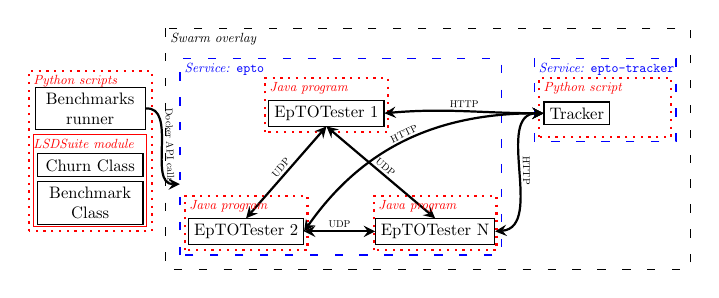
\begin{tikzpicture}[transform shape,scale=0.6]
\node[draw, text width=2.1cm, text centered] (bench) at (2.1, 2.6) {Benchmarks runner};

\draw (0.8,2.05) node[below right,red,scale=0.8] {\textit{LSDSuite module}};
\draw[red] (0.9,0.1) rectangle (3.3,2.05);
\node[draw, text width=2cm, text centered] (churnc) at (2.1,1.4) {Churn Class};
\node[draw, text width=2cm, text centered] (benchc) at (2.1, 0.6) {Benchmark Class};
\draw (0.8,3.4) node[below right,red,scale=0.8] {\textit{Python scripts}};
\draw[dotted,red,thick] (0.8,0) rectangle (3.4,3.4);
%
\draw[loosely dashed,black] (3.7,4.3) rectangle (14.8,-0.8);
\draw (3.7,4.3) node[below right,black,scale=0.8] {\textit{Swarm overlay}};
%
\node[draw] (tck) at (12.4, 2.5) {Tracker};
\draw (11.6,3.25) node[below right,red,scale=0.8] {\textit{Python script}};
\draw (11.5,3.65) node[below right,blue,scale=0.8] {\textit{Service:} \texttt{epto-tracker}};
\draw[loosely dashed,blue] (11.5,1.9) rectangle (14.5,3.65);
\draw[dotted,red,thick] (11.6,2) rectangle (14.4,3.25);
%
\draw[loosely dashed,blue] (4,-0.5) rectangle (10.8,3.65);
\draw (4,3.65) node[below right,blue,scale=0.8] {\textit{Service:} \texttt{epto}};
%
\node[draw] (app1) at (7.1, 2.5) {EpTOTester 1};
\draw (5.8,3.25) node[below right,red,scale=0.8] {\textit{Java program}};
\draw[dotted,red,thick] (5.8,2.1) rectangle (8.4,3.25);
%
\node[draw] (app2) at (5.4, 0) {EpTOTester 2};
\draw[dotted,red,thick] (4.1,-0.4) rectangle (6.7,.75);
%
\node[draw] (appn) at (9.4, 0) {EpTOTester N};
\draw[dotted,red,thick] (8.1,-0.4) rectangle (10.7,.75);
%
\draw[<->,thick,>=stealth] (app1.east) to[out=5,in=180] node[sloped,midway,scale=0.6,above]{HTTP} (tck.west);
\draw[<->,thick,>=stealth] (app2.east) to[out=55,in=180] node[sloped,midway,scale=0.6,above]{HTTP} (tck.west);
\draw[<->,thick,>=stealth] (appn.east) to[out=5,in=180] node[sloped,midway,scale=0.6,above]{HTTP} (tck.west);
%
\draw[->,thick,>=stealth] (bench.east) to[out=5,in=180] node[sloped,midway,scale=0.6,above]{Docker API calls} (4,1);
%
\draw[<->,thick,>=stealth] (app1.south) -- node[sloped,midway,scale=0.6,above]{UDP} (app2.north);
\draw[<->,thick,>=stealth] (app1.south) -- node[sloped,midway,scale=0.6,above]{UDP} (appn.north);
\draw[<->,thick,>=stealth] (app2.east) -- node[sloped,midway,scale=0.6,above]{UDP} (appn.west);
%
\draw (8.1,.75) node[below right,red,scale=0.8] {\textit{Java program}};
\draw (4.1,.75) node[below right,red,scale=0.8] {\textit{Java program}};
\end{tikzpicture} 
	\vspace{-2mm} 
	\caption{EpTOTester architecture}
	\vspace{-2mm} 
	\label{fig:complete-architecture}
\end{figure}
To deploy \epto effectively we need two different Docker Swarm services. One containing the tracker and one containing all \epto replicas. Both of these services use the same network overlay to communicate. This is achieved using Docker and especially the new Docker Swarm introduced in Docker 1.12. This lets us have a unified way of deploying our benchmarks locally or remotely on vastly different clusters with minimal modifications. Every benchmark is started through a Python script available on the master mode. This script handles everything from starting benchmarks, scaling the cluster during a churn and collecting results. All \epto parameters are customizable by using options provided through this script.
Gradle is used to automate the image building in the python scripts. Finally, a script is provided to push the images to a repository accessible to the remote cluster and to push the benchmarking script on the master node. \jgroups deployment is much the same. The entire EpTOTester architecture is shown in \autoref{fig:complete-architecture}. \jt{The figure is inspired from the one in ErasureBench. How should I indicate this?}
\subsection{Fault Injection}
Our framework supports the ability to inject synthetic and real traces thanks to the work done in \autocite{vaucher2016erasure}. The synthetic churn provided by it was improved to support adding and removing nodes at the same time.